\documentclass[12pt]{beamer}
\usepackage{../Estilos/BeamerFC}
\usepackage{../Estilos/ColoresLatex}
\usepackage{courier}
\usepackage{listingsutf8}
\usepackage{listings}
\usepackage{xcolor}
\usepackage{textcomp}
\usepackage{color}
\definecolor{deepblue}{rgb}{0,0,0.5}
\definecolor{brown}{rgb}{0.59, 0.29, 0.0}
\definecolor{OliveGreen}{rgb}{0,0.25,0}
% \usepackage{minted}

\DeclareCaptionFont{white}{\color{white}}
\DeclareCaptionFormat{listing}{\colorbox{gray}{\parbox{0.98\textwidth}{#1#2#3}}}
\captionsetup[lstlisting]{format=listing,labelfont=white,textfont=white}
\renewcommand{\lstlistingname}{Código}


\definecolor{Code}{rgb}{0,0,0}
\definecolor{Keywords}{rgb}{255,0,0}
\definecolor{Strings}{rgb}{255,0,255}
\definecolor{Comments}{rgb}{0,0,255}
\definecolor{Numbers}{rgb}{255,128,0}

\makeatletter

\newif\iffirstchar\firstchartrue
\newif\ifstartedbyadigit
\newif\ifprecededbyequalsign

\newcommand\processletter
{%
  \ifnum\lst@mode=\lst@Pmode%
    \iffirstchar%
        \global\startedbyadigitfalse%
      \fi
      \global\firstcharfalse%
    \fi
}

\newcommand\processdigit
{%
  \ifnum\lst@mode=\lst@Pmode%
      \iffirstchar%
        \global\startedbyadigittrue%
      \fi
      \global\firstcharfalse%
  \fi
}

\lst@AddToHook{OutputOther}%
{%
  \lst@IfLastOtherOneOf{=}
    {\global\precededbyequalsigntrue}
    {}%
}

\lst@AddToHook{Output}%
{%
  \ifprecededbyequalsign%
      \ifstartedbyadigit%
        \def\lst@thestyle{\color{orange}}%
      \fi
    \fi
  \global\firstchartrue%
  \global\startedbyadigitfalse%
  \global\precededbyequalsignfalse%
}

\lstset{ 
language=Python,                % choose the language of the code
basicstyle=\footnotesize\ttfamily,       % the size of the fonts that are used for the code
numbers=left,                   % where to put the line-numbers
numberstyle=\scriptsize,      % the size of the fonts that are used for the line-numbers
stepnumber=1,                   % the step between two line-numbers. If it is 1 each line will be numbered
numbersep=5pt,                  % how far the line-numbers are from the code
backgroundcolor=\color{white},  % choose the background color. You must add \usepackage{color}
showspaces=false,               % show spaces adding particular underscores
showstringspaces=false,         % underline spaces within strings
showtabs=false,                 % show tabs within strings adding particular underscores
frame=single,   		% adds a frame around the code
tabsize=2,  		% sets default tabsize to 2 spaces
captionpos=t,   		% sets the caption-position to bottom
breaklines=true,    	% sets automatic line breaking
breakatwhitespace=false,    % sets if automatic breaks should only happen at whitespace
escapeinside={| |},  % if you want to add a comment within your code
stringstyle =\color{OliveGreen},
otherkeywords={as, np.array, np.concatenate, np.linspace, linspace, interpolate.interp1d, kind, plt.plot, .copy, np.arange, np.cos, np.pi, lw, ls, label, splrep, splev, plt.legend, loc, plt.title, plt.ylim, plt.show, sign, math.ceil, math.log, np.sqrt, np.exp, np.zeros, plt.xlabel, plt.ylabel, plt.xlim, np.identity, random, np.dot, np.outer, np.diagonal },             % Add keywords here
keywordstyle = \color{blue},
commentstyle = \color{darkcerulean},
identifierstyle = \color{black},
literate=%
         {á}{{\'a}}1
         {é}{{\'e}}1
         {í}{{\'i}}1
         {ó}{{\'o}}1
         {ú}{{\'u}}1
%
%keywordstyle=\ttb\color{deepblue}
%fancyvrb = true,
}

\lstdefinestyle{FormattedNumber}{%
    literate={0}{{\textcolor{red}{0}}}{1}%
             {1}{{\textcolor{red}{1}}}{1}%
             {2}{{\textcolor{red}{2}}}{1}%
             {3}{{\textcolor{red}{3}}}{1}%
             {4}{{\textcolor{red}{4}}}{1}%
             {5}{{\textcolor{red}{5}}}{1}%
             {6}{{\textcolor{red}{6}}}{1}%
             {7}{{\textcolor{red}{7}}}{1}%
             {8}{{\textcolor{red}{8}}}{1}%
             {9}{{\textcolor{red}{9}}}{1}%
             {.0}{{\textcolor{red}{.0}}}{2}% Following is to ensure that only periods
             {.1}{{\textcolor{red}{.1}}}{2}% followed by a digit are changed.
             {.2}{{\textcolor{red}{.2}}}{2}%
             {.3}{{\textcolor{red}{.3}}}{2}%
             {.4}{{\textcolor{red}{.4}}}{2}%
             {.5}{{\textcolor{red}{.5}}}{2}%
             {.6}{{\textcolor{red}{.6}}}{2}%
             {.7}{{\textcolor{red}{.7}}}{2}%
             {.8}{{\textcolor{red}{.8}}}{2}%
             {.9}{{\textcolor{red}{.9}}}{2}%
             {\ }{{ }}{1}% handle the space
         ,%
          %mathescape=true
          escapeinside={__}
          }



\usetheme{Copenhagen}
\usecolortheme{wolverine}
%\useoutertheme{default}
\setbeamercovered{invisible}
% or whatever (possibly just delete it)
\setbeamertemplate{section in toc}[sections numbered]
\setbeamertemplate{subsection in toc}[subsections numbered]
\setbeamertemplate{subsection in toc}{\leavevmode\leftskip=3.2em\rlap{\hskip-2em\inserttocsectionnumber.\inserttocsubsectionnumber}\inserttocsubsection\par}
% \setbeamercolor{section in toc}{fg=blue}
% \setbeamercolor{subsection in toc}{fg=blue}
% \setbeamercolor{frametitle}{fg=blue}
\setbeamertemplate{caption}[numbered]

\setbeamertemplate{footline}
\beamertemplatenavigationsymbolsempty
\setbeamertemplate{headline}{}


\makeatletter
% \setbeamercolor{section in foot}{bg=gray!30, fg=black!90!orange}
% \setbeamercolor{subsection in foot}{bg=blue!30}
% \setbeamercolor{date in foot}{bg=black}
\setbeamertemplate{footline}
{
  \leavevmode%
  \hbox{%
  \begin{beamercolorbox}[wd=.333333\paperwidth,ht=2.25ex,dp=1ex,center]{section in foot}%
    \usebeamerfont{section in foot} \insertsection
  \end{beamercolorbox}%
  \begin{beamercolorbox}[wd=.333333\paperwidth,ht=2.25ex,dp=1ex,center]{subsection in foot}%
    \usebeamerfont{subsection in foot}  \insertsubsection
  \end{beamercolorbox}%
  \begin{beamercolorbox}[wd=.333333\paperwidth,ht=2.25ex,dp=1ex,right]{date in head/foot}%
    \usebeamerfont{date in head/foot} \insertshortdate{} \hspace*{2em}
    \insertframenumber{} / \inserttotalframenumber \hspace*{2ex} 
  \end{beamercolorbox}}%
  \vskip0pt%
}
\makeatother

\makeatletter
\patchcmd{\beamer@sectionintoc}{\vskip1.5em}{\vskip0.8em}{}{}
\makeatother

% %\newlength{\depthofsumsign}
% \setlength{\depthofsumsign}{\depthof{$\sum$}}
% \newcommand{\nsum}[1][1.4]{% only for \displaystyle
%     \mathop{%
%         \raisebox
%             {-#1\depthofsumsign+1\depthofsumsign}
%             {\scalebox
%                 {#1}
%                 {$\displaystyle\sum$}%
%             }
%     }
% }
% \def\scaleint#1{\vcenter{\hbox{\scaleto[3ex]{\displaystyle\int}{#1}}}}
% \def\scaleoint#1{\vcenter{\hbox{\scaleto[3ex]{\displaystyle\oint}{#1}}}}
% \def\bs{\mkern-12mu}

% \usefonttheme{serif}

\title{\large{Ecuaciones Diferenciales Ordinarias}}
\subtitle{Tema 3 - Ecuaciones Diferenciales Ordinarias}
\author{M. en C. Gustavo Contreras Mayén}
\date{}

\begin{document}
\maketitle

\section*{Contenido}
\frame{\tableofcontents[currentsection, hideallsubsections]}

\section{Las EDO}
\frame{\tableofcontents[currentsection, hideothersubsections]}
\subsection{Breve repaso}

\begin{frame}
\frametitle{Introducción}
Las ecuaciones diferenciales tienen importancia fundamental en las aplicaciones, ya que muchas leyes y relaciones físicas pueden expresarse matemáticamente de esta forma.
\\
\medskip
\pause
En particular, el estudio de problemas de equilibrio de sistemas continuos se encuentra dentro de este contexto.
\end{frame}
\begin{frame}
\frametitle{Definiciones importantes}
\begin{block}{Aviso de consideración}
No sería mala idea hacer un repaso en casa sobre estas definiciones y los métodos analíticos de solución de las	\textit{Ecuaciones Diferenciales Ordinarias} EDO.
\end{block}
\end{frame}
\begin{frame}
\frametitle{Ecuación diferencial}
Esta ecuación relaciona dos o más variables en términos de derivadas o diferenciales.
\pause
\begin{eqnarray*}
\begin{aligned}
\dv{y}{x} &= \cos x \\ \pause
\dv[2]{y}{x} &= \cos x \\ \pause
( x^{2} + y^{2} ) \dd{x} + 2 \, x \, y \dd{y} &= 0 \\ \pause
\left[ \dv[2]{w}{x} \right]^{3} - x \, y \, \dv{w}{x} &= 0 
\end{aligned}
\end{eqnarray*}
\end{frame}
\begin{frame}
\frametitle{Ecuaciones diferenciales ordinarias (EDO) y parciales}
Si en una ecuación diferencial hay una sola variable independiente, las derivadas son totales y se le llama \textit{ecuación ordinaria}.
\\
\medskip
\pause
Si en la ecuación hay dos o más variables independientes, las derivadas serán parciales y se le llama \textit{ecuación parcial}.
\begin{align*}
\pdv[2]{V}{x} + \pdv[2]{V}{y} = 0
\end{align*}
\end{frame}
\begin{frame}
\frametitle{Orden de una ecuación diferencial}
Es la derivada de mayor orden que aparece en la ecuación.
\end{frame}
\begin{frame}
\frametitle{Grado de una ecuación diferencial}
Es el grado \textit{algebraico} de la derivada de mayor orden que aparece en la ecuación.
\end{frame}
\begin{frame}
\frametitle{Ecuación diferencial lineal}
Una ecuación diferencial es lineal si en ella no aparecen potencias de la variable dependiente y sus derivadas, ni productos de la variable dependiente por sus derivadas o productos entre derivadas.
\end{frame}
\begin{frame}
\frametitle{Solución de una ecuación diferencial}
Es cualquier relación funcional que no incluya derivadas o integrales de funciones desconocidas y que implique a la propia ecuación diferencial, en el sentido de que la verifique por sustitución directa.
\end{frame}
\begin{frame}
\frametitle{Ecuación y condiciones homogéneas}
Una ecuación o condición es homogénea si, cuando es satisfecha por una función particular $y (x)$, también es satisfecha por $c \, y(x)$, donde $c$ es una constante arbitraria.
\end{frame}
\begin{frame}
\frametitle{Solución de una ecuación diferencial}
Sea una ecuación diferencial ordinaria de orden $n$ y cualquier grado, cuya forma más general es:
\pause
\begin{align*}
F (x, y, \pderivada{y}, \sderivada{y}, \ldots, y^{(n)}) = 0
\end{align*}
\pause
Se establece del cálculo que en su solución general deben de aparecer $n$ constantes arbitrarias. \pause Entonces puede aceptarse como solución general:
\pause
\begin{align*}
G (x,y , c_{1}, c_{2}, \ldots, c_{n}) = 0
\end{align*}
\end{frame}
\begin{frame}[fragile]
\frametitle{Solución de una EDO}
\begin{tikzpicture}[font=\small]
	\draw [->] (0, 0) -- (7, 0);
	\draw [->] (0, 0) -- node [near end, left] {$y$} (0, 5);
	\draw (1, 1) .. controls (2.5, 2.5) and (4, 3) .. (6, 3);
	\draw (1, 2) .. controls (2.5, 3.5) and (4, 4) .. (6, 4);
	\draw (1, 0.2) .. controls (2.5, 1.7) and (4, 2.2) .. (6, 2.2);
	\draw (7.3 ,-0.1) node {$x$};
	\draw (7.2, 2.2) node {$G_{1} = 0$};
	\draw (7.2, 4.2) node {$G_{2} = 0$};
	\draw (7.2, 3.2) node {$G_{3} = 0$};
\end{tikzpicture}
\end{frame}
\begin{frame}
\frametitle{Ejemplo}
Gráficamente esta ecuación representa a una familia de curvas planas, cada una de ellas obtenidas para valores particulares de las $n$ constantes $c_{1}, c_{2}, \ldots, c_{n}$
\end{frame}
\begin{frame}
\frametitle{Tipos de problemas}
Dependiendo de cómo se establezcan estas condiciones, se distinguen dos tipos de problemas los llamados {\color{red}\textit{de valores iniciales}} y los {\color{ao}\textit{de valores en la frontera}}.
\end{frame}
\begin{frame}
\frametitle{Problemas de valores iniciales}
Está gobernado por una ecuación diferencial de orden $n$ y un conjunto de $n$ condiciones independientes, todas ellas válidas para el mismo punto inicial.
\end{frame}
\begin{frame}
\frametitle{Problemas de valores iniciales}
Si la ecuación diferencial que define el problema es del tipo de la EDO con la que iniciamos y $x = a$ es el punto inicial, puede aceptarse que las $n$ condiciones independientes son:
\end{frame}
\begin{frame}
\frametitle{$n$ condiciones independientes}
\begin{eqnarray*}
\begin{aligned}
y(a) & = y_{0} \\ \pause
\pderivada{y} (a) & = \pderivada{y}_{0} \\ \pause
\sderivada{y} (a) & = \pderivada{y}_{0} \\ \pause
\vdots \\
y^{(n)} (a) & = y^{(n)}_{0} 
\end{aligned}
\end{eqnarray*}
Se tratará de obtener una solución particular de la EDO inicial que verifique las condiciones iniciales, como se presenta en la siguiente figura:
\end{frame}
\begin{frame}[fragile]
\frametitle{Solución de una EDO con condiciones inciales}
\begin{tikzpicture}[font=\small]
	\draw [->] (0, 0) -- (7, 0);
	\draw [->] (0, 0) -- node [near end, left] {$y$} (0, 5);
	\draw (1, 2) .. controls (2.5, 3.5) and (4, 4) .. (6, 4);
	\draw (7.3, -0.1) node {$x$};
	\draw (7.2, 4.2) node {$g(x, y) = 0$};
	\draw [dashed] (1.5, 0) -- (1.5, 2.4);
	\draw (1.3, -0.2) node {$x = a$};
\end{tikzpicture}
\end{frame}
\begin{frame}
\frametitle{Problemas de valores en la frontera}
Se deben de establecer condiciones de frontera en todos y cada uno de los puntos que constituyen la frontera del dominio de soluciones del problema.
\\
\medskip
\pause
En particular, en el espacio de una dimensión, hay dos puntos frontera, por ejemplo $x = a$ y $x = b$ si el dominio de soluciones es el intervalo cerrado $a \leq x \leq b$
\end{frame}
\begin{frame}[fragile]
\frametitle{Solución de una EDO con condiciones de frontera}
\begin{tikzpicture}[font=\small]
	\draw [->] (0, 0) -- (7, 0);
	\draw [->] (0, 0) -- node [near end, left] {$y$} (0, 5);
	\draw (1, 2) .. controls (2.5, 3.5) and (4,4) .. (6, 4);
	\draw (7.3, -0.1) node {$x$};
	\draw (7.2, 4.2) node {$g(x, y) = 0$};
	\draw [dashed] (1.5, 0) -- (1.5, 2.4);
	\draw (1.3, -0.2) node {$x = a$};
	\draw [dashed] (5.2, 0) -- (5.2, 4);
	\draw (5, -0.2) node {$x = b$};
\end{tikzpicture}
\end{frame}
\begin{frame}
\frametitle{Estrategia de solución}
Básicamente la solución numérica de las ecuaciones diferenciales consiste en sustituir el dominio continuo de soluciones por uno discreto formado por puntos aislados igualmente espaciados entre sí.
\end{frame}
\begin{frame}
\frametitle{Problema de valores iniciales}
El dominio de definición de soluciones $x \geq a$  se sustituye por el conjunto infinito numerable de puntos:
\pause
\begin{eqnarray*}
\begin{aligned}
x_{0} & = a \\ \pause
x_{1} & = x_{0} + h \\ \pause
x_{2} & = x_{0} + 2 \, h \\ \pause
x_{3} & = x_{0} + 3 \, h \\ \pause
\ldots
\end{aligned}
\end{eqnarray*}
\end{frame}
\begin{frame}[fragile]
\frametitle{Valores inciales}
\begin{tikzpicture}[font=\small]
	\draw [->] (0, 0) -- (7, 0);
	\draw [->] (0, 0) -- node [near end, left] {$y$} (0, 5);
	\draw (1, 2) .. controls (2.5, 3.5) and (4, 4) .. (6, 4);
	\draw (7.3, -0.1) node {$x$};
	\draw (7.2, 4.2) node {$g (x, y) = 0$};
	\draw [dashed] (1.5, 0) -- (1.5, 2.4);
	\draw (1.3, -0.2) node {$x_{0} = a$};
	\draw [dashed] (2.3, 0) -- (2.3, 3.15);
	\draw (2.3, -0.2) node {$x_{1}$};
	\draw [dashed] (3.3, 0) -- (3.3, 3.6);
	\draw (3.3, -0.2) node {$x_{2}$};
	\draw [dashed] (4.3, 0) -- (4.3, 3.85);
	\draw (4.3, -0.2) node {$x_{3}$};
	\draw (5.3, -0.2) node {$\ldots$};
\end{tikzpicture}
\end{frame}
\begin{frame}
\frametitle{Problema de valores en la frontera}
Se sustituye el intervalo $a \leq x \leq b $ por el conjunto finito de puntos:
\pause
\begin{eqnarray*}
\begin{aligned}
x_{0} & = a \\ \pause
x_{1} & = x_{0} + h \\ \pause
x_{2} & = x_{0} + 2 \, h \\ \pause
x_{3} & = x_{0} + 3 \, h \\ \pause
\ldots \\
x_{n} & = x_{0} + n \, h = b
\end{aligned}
\end{eqnarray*}
\end{frame}
\begin{frame}[fragile]
\frametitle{Valores en la frontera}
\begin{tikzpicture}[font=\small]
	\draw [->] (0, 0) -- (7, 0);
	\draw [->] (0, 0) -- node [near end, left] {$y$} (0, 5);
	\draw (1, 2) .. controls (2.5, 3.5) and (4, 4) .. (6, 4);
	\draw (7.3, -0.1) node {$x$};
	\draw (7.2, 4.2) node {$g (x, y) = 0$};
	\draw [dashed] (1.5, 0) -- (1.5, 2.4);
	\draw (1.3, -0.2) node {$x_{0} = a$};
	\draw [dashed] (2.3, 0) -- (2.3, 3.15);
	\draw (2.3, -0.2) node {$x_{1}$};
	\draw [dashed] (3.3, 0) -- (3.3, 3.6);
	\draw (3.3, -0.2) node {$x_{2}$};
	\draw [dashed] (4.3, 0) -- (4.3, 3.85);
	\draw (4.3, -0.2) node {$x_{3}$};
	\draw (5.1, -0.2) node {$\ldots$};
	\draw [dashed] (5.9, 0) -- (5.9, 4);
	\draw (6, -0.2) node {$x_{n} = b$};
\end{tikzpicture}
\end{frame}
\begin{frame}
\frametitle{Nuestra tarea}
Una vez discretizado el problema continuo, se tratará de obtener la solución para los puntos considerados, esto se resuelve en general, sustituyendo las derivadas que aparezcan en la ecuación diferencial y en sus condiciones iniciales o de frontera.
\end{frame}
\begin{frame}
\frametitle{Nuestra tarea}
Usando fórmulas numéricas de derivación que proporcionen una aproximación a las derivadas o tratando de integrar la ecuación, reemplazando el proceso de integración por una fórmula numérica que se aproxime a la integral.
\end{frame}

\section{Problemas de valores iniciales}
\frame{\tableofcontents[currentsection, hideothersubsections]}
\subsection{Definición}

\begin{frame}
\frametitle{Problemas de valores iniciales}
Debemos de resolver el problema:
\pause
\begin{align*}
\pderivada{y} = F (x, y)
\end{align*}
con la condición auxiliar $y (a) = \alpha$
\end{frame}
\begin{frame}
\frametitle{Forma general de una EDO de 1er. orden}
La forma general de una ecuación diferencial de primer orden (EDO1) es:
\begin{align*}
\pderivada{y} = f (x, y)
\end{align*}
donde $\pderivada{y} = \dv*{y}{x}$ y $f (x, y)$ es una función dada.
\end{frame}
\begin{frame}
\frametitle{Forma general de una EDO de 1er. orden}
La solución de esta ecuación incluye una constante arbitraria (la constante de integración); \pause para hallar esa constante, debemos conocer un punto en la curva solución, esto es, $y$ debe de especificarse para algún valor de $x$, $x = a$. 
\\
\bigskip
\pause
Entonces, escribimos, la condición auxiliar $y (a) = \alpha$
\end{frame}
\begin{frame}
\frametitle{Reducción de orden en la EDO}
Una ecuación diferencial de orden $n$:
\pause
\begin{align*}
y^{(n)} = f (x, y, \pderivada{y}, \ldots, y^{(n-1)})
\end{align*}
\pause
se puede transformar en un conjunto de $n$ ecuaciones diferenciales de primer orden; usemos la notación:
\pause
\begin{alignat*}{5}
y_{0} & = y & y_{1} & = \pderivada{y} \\
y_{2} & = \sderivada{y} & y_{3} & = \tderivada{y} \\
\ldots & & &  \\ 
y_{n-1} & = y^{(n-1)} & & 
\end{alignat*}
\end{frame}
\begin{frame}
\frametitle{EDO con orden reducido}
Las ecuaciones EDO1 equivalentes son:
\pause
\begin{eqnarray*}
\begin{aligned}
\pderivada{y}_{0} &= y_{1} \\
\pderivada{y}_{1} &= y_{2} \\
\pderivada{y}_{2} &= y_{3} \\
\ldots \\
\pderivada{y}_{n} &= f (x, y_{0}, y_{1}, \ldots, y_{n - 1})
\end{aligned}
\end{eqnarray*}
\end{frame}
\begin{frame}
\frametitle{Condiciones iniciales}
La solución ahora requiere de $n$ condiciones auxiliares; si esas condiciones se especifican para el mismo valor de $x$, el problema se dice que es \emph{\textocolor{blue}{un problema de valores iniciales}}.
\\
\medskip
\pause
Las condiciones auxiliares, se llaman \emph{\textocolor{lava!90!black}{condiciones iniciales}}, que tienen la forma:
\pause
\begin{align*}
y_{0} (a) = \alpha_{0} \hspace{0.5cm} y_{1} (a) = \alpha_{1} \hspace{0.5cm} \ldots \hspace{0.5cm} y_{n-1} (a) = \alpha_{n-1}
\end{align*}
\end{frame}
\begin{frame}
\frametitle{Tipos de problemas}
Si $y_{i}$ se especifica para diferentes valores de $x$, el problema se llama \emph{problema con condiciones de frontera}, por ejemplo:
\pause
\begin{align*}
\sderivada{y} = - y \hspace{1cm} y (0) = 1 \hspace{1cm} \pderivada{y} (\pi) = 0
\end{align*}
es un \textocolor{awesome}{problema con condiciones de frontera}, ya que las dos condiciones se cumplen para diferentes valores de $x$.
\end{frame}
\begin{frame}
\frametitle{Tipos de problemas}
Mientras que:
\pause
\begin{align*}
\sderivada{y} = -y \hspace{1cm} y (0) = 1 \hspace{1cm} \pderivada{y} (0) = 0
\end{align*}
es un \textocolor{bole}{problema de condiciones iniciales}, ya que ambas condiciones están definidas en la solución para $x = 0$.
\end{frame}
\begin{frame}
\frametitle{Notación usada para el tema EDO}
Se usará de manera continua y por conveniencia, la notación vectorial, que nos permitirá manejar conjuntos de EDO1 de una manera más clara, de tal manera que podremos expresar:
\pause
\renewcommand*{\arraystretch}{0.7}
\begin{eqnarray*}
\begin{aligned}
\mathbf{\pderivada{y}} = \mathbf{F} (x, \mathbf{y}) \hspace{1.3cm} \mathbf{y} (a) = \alpha \hspace{1cm}
\mathbf{F} (x, \mathbf{y}) = \left[ \begin{matrix}
y_{1} \\
y_{2} \\
\ldots \\
f (x, \mathbf{y})
\end{matrix} \right]
\end{aligned}
\end{eqnarray*}
\end{frame}

\section{Método de Euler}
\frame[allowframebreaks]{\tableofcontents[currentsection, hideothersubsections]}
\subsection{Construcción}

\begin{frame}
\frametitle{Método de Euler}
El método de Euler tiene una base muy sencilla: \pause se trunca la serie de Taylor para $\mathbf{y}$ alrededor de $x$:
\begin{align*}
\mathbf{y} (x + h) \approx \mathbf{y} (x) + \pderivada{\mathbf{y}} (x) \, h
\end{align*}
La expresión anterior predice el valor de $\mathbf{y}$ en $x + h$ con la información disponible de $x$, se puede usar para avanzar la solución en pasos de $h$, comenzando con los valores iniciales dados de $x$ e $\mathbf{y}$.
\end{frame}
\begin{frame}
\frametitle{Error de truncamiento}
El error debido al truncamiento, es:
\pause
\begin{align*}
\mathbf{E} = \dfrac{1}{2} \, \sderivada{y} (\xi) \, h^{2} = \order{h^{2}}, \hspace{0.7cm} x < \xi < x + h
\end{align*}
\end{frame}
\begin{frame}
\frametitle{Error de truncamiento}
Se puede obtener una idea aproximada del error acumulado $\mathbf{E}_{\text{acc}}$ suponiendo que el error por paso es constante durante el período de integración.
\end{frame}
\begin{frame}
\frametitle{Error de truncamiento}
Luego, después de $n$ pasos de integración que cubren el intervalo $x_{0}$ a $x_{n}$, tenemos:
\pause
\begin{align*}
\mathbf{E}_{\text{acc}} = n \, \mathbf{E} = \dfrac{x_{n} - x_{0}}{h} \, \mathbf{E} = \order{h}
\end{align*}
Por lo tanto, el error acumulado es un orden menor que el error por paso.
\end{frame}
\begin{frame}
\frametitle{Interpretación de la fórmula de Euler}
Veamos ahora la interpretación gráfica de la ecuación de Euler.
\\
\bigskip
\pause
En aras de la simplicidad, asumimos que hay un sola variable dependiente $y$, de modo que la ecuación diferencial es:
\begin{align*}
\pderivada{y} = f (x, y)
\end{align*}
\end{frame}
\begin{frame}
\frametitle{Interpretación de la fórmula de Euler}
El cambio en la solución $y$ entre $x$ y $x + h$ es:
\pause
\begin{align*}
y (x + h) - y (h) = \scaleint{6ex}_{\bs x}^{x+h} \pderivada{y} \dd{x} = \scaleint{6ex}_{\bs x}^{x+h} f (x, y) \dd{x}
\end{align*}
que es el área del panel bajo la gráfica $\pderivada{y} (x)$, que se muestra en la siguiente figura.
\end{frame}
\begin{frame}[fragile]
\frametitle{Interpretación de la fórmula de Euler}
\begin{figure}
    \centering
    \begin{tikzpicture}[font=\small]
        \draw [->] (0, 0) -- (7, 0);
        \draw [->] (0, 0) -- node [pos=1, left] {$\pderivada{y} (x)$} (0, 5);
        \draw (1, 2) .. controls (2.5, 3.5) and (4,4) .. (6, 4);
        \draw (7.3, -0.1) node {$x$};
        \draw (7.2, 4.2) node {$f (x, y)$};
        \draw [dashed] (1.5, 0) -- (1.5, 2.4);
        \draw (1.3, -0.2) node {$x$};
        \draw [dashed] (5.2, 0) -- (5.2, 4);
        \draw (5, -0.2) node {$x + h$};
        \draw [pattern=north west lines, pattern color=blue] (1.5, 0) rectangle (5.2, 2.45);
        \node at (7.2, 3) {Error truncamiento};
        \draw [->, thick] (5.5, 3) -- (3.5, 3);
        \node at (7.2, 1) {Fórmula de Euler};
        \draw [->, thick] (5.6, 1) -- (3, 1);
    \end{tikzpicture}
\end{figure}
\end{frame}
\begin{frame}
\frametitle{Aproximación de Euler}
La fórmula de Euler aproxima esta área por el área del rectángulo rayado.
\\
\bigskip
\pause
El área entre el rectángulo y la gráfica representa el error de truncamiento. \pause Claramente, el error de truncamiento es proporcional a la pendiente de la gráfica; es decir, es proporcional a $(\pderivada{y})^{\prime} = \sderivada{y} (x)$.
\end{frame}
\begin{frame}
\frametitle{Desventaja del método de Euler}
El método de Euler rara vez se usa en la práctica debido a su ineficiencia computacional.
\\
\bigskip
\pause
Suprimir el error de truncamiento a un nivel aceptable requiere una $h$ muy pequeña, lo que da como resultado muchos pasos de integración acompañados de un aumento en el error de redondeo.
\end{frame}
\begin{frame}
\frametitle{Utilidad del método de Euler}
El valor del método radica principalmente en su simplicidad, que facilita la discusión de ciertos temas importantes, como la estabilidad.
\end{frame}

\subsection{Ejercicio 1}

\begin{frame}
\frametitle{Ejercicio 1}
Integra el problema de valor inicial:
\pause
\begin{align*}
\pderivada{y} + 4 \, y = x^{2} \hspace{1.5cm} y(0) = 1
\end{align*}
en pasos de $h = 0.01$ de $x = 0$ a $0.03$
\pause
Calcula:
\setbeamercolor{item projected}{bg=blush,fg=white}
\setbeamertemplate{enumerate items}{%
\usebeamercolor[bg]{item projected}%
\raisebox{1.5pt}{\colorbox{bg}{\color{fg}\footnotesize\insertenumlabel}}%
}
\begin{enumerate}[<+->]
\item La solución analítica $y (x)$.
\item El error acumulado en cada paso.
\end{enumerate}
\end{frame}
\begin{frame}
\frametitle{Solución analítica}
La solución analítica de la EDO1 es:
\pause
\begin{align*}
y =  \dfrac{31}{32} \exp(-4 x) + \dfrac{1}{4} x^{2} - \dfrac{1}{8} x + \dfrac{1}{32}
\end{align*}
\end{frame}
\begin{frame}
\frametitle{Solución al Ejercicio 1}
Es conveniente usar la notación:
\pause
\begin{align*}
x_{i} = i \, h \hspace{1cm} y_{i} = y (x_{i})
\end{align*}
\pause
Por lo que la fórmula de Euler toma la forma:
\pause
\begin{align*}
y_{i+1} = y_{i} + \pderivada{y}_{i} \, h
\end{align*}
donde:
\begin{align*}
\pderivada{y}_{i} = x_{i}^{2} - 4 \, y_{i}
\end{align*}
\end{frame}
\begin{frame}
\frametitle{Paso 1}
De $x_{0} = 0$ a $x_{1} = 0.01$:
\pause
\begin{eqnarray*}
\begin{aligned}
y_{0} &= 1 \\ \pause
\pderivada{y}_{0} &= x_{0}^{2} - 4 \, y_{0} = 0^{2} - 4 (1) = \pause - 4 \\ \pause
y_{1} &= y_{0} + \pderivada{y} \, h = \pause 1 + (-4)(0.01) = \pause = 0.96 \\ \pause
(y_{1})_{\text{exacta}} &= \dfrac{31}{32} \exp(-4 (0.01)) + \dfrac{1}{4} (0.01)^{2} - \dfrac{1}{8} (0.01) +  \\
&+ \dfrac{1}{32} = \pause 0.9608 \\ \pause
\text{E}_{\text{acum}} &= 0.96 - 0.9608 = \pause -0.0008
\end{aligned}
\end{eqnarray*}
\end{frame}
\begin{frame}
\frametitle{Paso 2}
De $x_{0} = 0.01$ a $x_{1} = 0.02$:
\pause
\begin{eqnarray*}
\begin{aligned}
\pderivada{y}_{1} &= \pause x_{1}^{2} - 4 \, y_{1} = \pause 0.01^{2} - 4 (0.96) = \pause - 3.840 \\ \pause
y_{2} &= y_{1} + \pderivada{y}_{1} \, h = \pause 0.96 + (- 3.840)(0.01) = \pause = 0.9216 \\ \pause
(y_{2})_{\text{exacta}} &= \dfrac{31}{32} \exp(-4 (0.02)) + \dfrac{1}{4} (0.02)^{2} - \dfrac{1}{8} (0.02) +  \\
&+ \dfrac{1}{32} = \pause 0.9231 \\ \pause
\text{E}_{\text{acum}} &= 0.9216 - 0.9231 = \pause -0.0015
\end{aligned}
\end{eqnarray*}
\end{frame}
\begin{frame}
\frametitle{Paso 3}
De $x_{0} = 0.02$ a $x_{1} = 0.03$:
\pause
\begin{eqnarray*}
\begin{aligned}
\pderivada{y}_{2} &= \pause x_{2}^{2} - 4 \, y_{2} = \pause 0.02^{2} - 4 (0.9216) = \pause - 3.686 \\ \pause
y_{3} &= y_{2} + \pderivada{y}_{2} \, h = \pause 0.92616 + (- 3.686)(0.01) = \pause = 0.8847 \\ \pause
(y_{3})_{\text{exacta}} &= \dfrac{31}{32} \exp(-4 (0.03)) + \dfrac{1}{4} (0.03)^{2} - \dfrac{1}{8} (0.03) +  \\
&+ \dfrac{1}{32} = \pause 0.8869 \\ \pause
\text{E}_{\text{acum}} &= 0.8847 - 0.8869 = \pause -0.0022
\end{aligned}
\end{eqnarray*}
\end{frame}
\begin{frame}
\frametitle{Sobre el error}
Notamos que la magnitud del error por paso es aproximadamente constante en $0.008$.
\\
\bigskip
\pause
Por lo tanto, después de $10$ pasos de integración, el error acumulado sería de aproximadamente $0.008$, lo que reduciría la precisión de la solución a una cifra significativa. \pause Después de $100$ pasos, se perderían todas las cifras significativas.
\end{frame}


\subsection{módulo \texttt{Métodos Directos}}

\begin{frame}
\frametitle{Módulo con las funciones}
En este Tema 3, debermos de incluir todas las funciones de los métodos directos para resolver una EDO en el módulo \funcionazul{metodosDirectos}.
\\
\bigskip
\pause
Haciendo la debida llamada al módulo y función(es) que se necesiten para cada ejercicio.
\end{frame}
\begin{frame}
\frametitle{Manejo de los módulo}
Cuiden que la ruta del módulo se encuentre bien identificada para evitar errores de que no reconoce el nombre de la función y/o módulo.
\end{frame}

\subsection{Función \texttt{Euler}}

\begin{frame}
\frametitle{La función \texttt{Euler}}
Esta función implementa el \textocolor{ao}{método de integración de Euler}.
\\
\bigskip
\pause
Puede manejar cualquier número de ecuaciones diferenciales de primer orden.
\end{frame}
\begin{frame}
\frametitle{La función \texttt{Euler}}
El usuario debe proporcionar la función \funcionazul{F (x, y)} que especifica las ecuaciones diferenciales en forma de arreglo:
\pause
\renewcommand*{\arraystretch}{0.7}
\begin{align*}
\mathbf{F} (x, \mathbf{y}) = 
\begin{bmatrix}
\pderivada{y}_{0} \\
\pderivada{y}_{1} \\
\pderivada{y}_{2} \\
\vdots
\end{bmatrix}
\end{align*}
\end{frame}
\begin{frame}
\frametitle{Lo que devuelve la función}
La función devuelve los arreglos \texttt{X} y \texttt{Y} que contienen los valores de $x$ y de $y$ en intervalos $h$.
\end{frame}
\begin{frame}[allowframebreaks, fragile]
\begin{lstlisting}[caption=Método de Euler]
import numpy as np

def euler(F, x, y, xAlto, h):
    X = []
    Y = []
    X.append(x)
    Y.append(y)

    while x < xAlto:
        h = min(h, xAlto - x)
        y = y + h * F(x, y)
        x = x + h
        X.append(x)
        Y.append(y)

    return np.array(X), np.array(Y)
\end{lstlisting}
\end{frame}
\begin{frame}
\frametitle{Solución con código}
Con el mismo ejercicio que acabamos de resolver paso a paso, ahora trabajaremos con un código con el que podremos extender el número de elementos para el sistema de EDO1.
\end{frame}
\begin{frame}[allowframebreaks, fragile]
\frametitle{Código para el Ejercicio 1}
\begin{lstlisting}[caption=Código para resolver la EDO1]
from metodosDirectos import euler
from prettytable import PrettyTable
import numpy as np

def f(x, y):
	f = np.zeros(1)
	f[0] = x**2 - 4 * y
	return f

def s_Exacta(x):
	valor = (31/32.) * np.exp(-4*x) + (1/4.) * x**2 - (1/8.) *x + (1/32.)
	return valor

x = 0.0
xAlto = 0.03
y = np.array([1.])
h = 0.01

X, Y = euler(f, x, y, xAlto, h)

tabla = PrettyTable()
tabla.field_names = ['x', 'Aproximacion', 'Exacta', 'Error']

for i in range(1, len(Y)):
	diferencia = s_Exacta(X[i]) - Y[i]
	tabla.add_row([X[i], '%1.4f' % Y[i], '%1.4f' % s_Exacta(X[i]), '%1.4f:' % diferencia])
	
print(tabla)
\end{lstlisting}
\end{frame}

\subsection{Ejercicio 2}

\begin{frame}
\frametitle{Ejercicio 2}
Integra el problema de valores iniciales:
\begin{align*}
\sderivada{y} = -0.1 \, \pderivada{y} - x \hspace{0.75cm} y (0) = 0 \hspace{0.5cm} \pderivada{y} (0) = 1
\end{align*}
de $x = 0$ hasta $x = 2$ con el método de Euler, usando $h = 0.05$. Genera una gráfica de las soluciones aproximada y la analítica.
\pause
\begin{align*}
y (x) = 100 \, x - 5 \, x^{2} + 990 \big( e^{-0.1 x} - 1 \big)
\end{align*}
\end{frame}
\begin{frame}
\frametitle{Solución al ejercicio 2}
Usemos la notación $y_{0} = y$ y $y_{1} = \pderivada{y}$ para un conjunto de EDO1, con las condiciones iniciales:
\pause
\begin{align*}
\mathbf{F} (x, \mathbf{y}) = \begin{bmatrix}
\pderivada{y}_{0} \\
\pderivada{y}_{1}
\end{bmatrix}
=
\begin{bmatrix}
y[1] \\
-0.1 \, y[1] - x
\end{bmatrix}
\hspace{1.5cm}
\mathbf{y} (0) =
\begin{bmatrix}
0 \\
1
\end{bmatrix}
\end{align*}
\end{frame}
\begin{frame}
\frametitle{Archivo nuevo para la solución}
Recuerda que en cada ejercicio se recomienda ampliamente generar un archivo nuevo con código.
\\
\bigskip
\pause
Ya conoces las rutinas necesarias para presentar una gráfica, por lo que deberás de incluir las correspondientes librerías y funciones.
\end{frame}
\begin{frame}[allowframebreaks, fragile]
\frametitle{Código para el Ejercicio 2}
\begin{lstlisting}[caption=Código para resolver el ejercicio con el método de Euler]
from metodosDirectos import euler
import numpy as np

def f(x, y):
	f = np.zeros(2)
	f[0] = y[1]
	f[1] = -0.1 * y[1] - x
	return f

x = 0.0
xAlto = 2.0
y = np.array([0., 1.])
h = 0.05

X, Y = euler(f, x, y, xAlto, h)

s_Exacta = 100. * X - 5. * X**2 + 990. *(np.exp(-0.1 * X) - 1.)
\end{lstlisting}
\end{frame}
\begin{frame}
\frametitle{Gráfica obtenida}
\begin{figure}
	\centering
	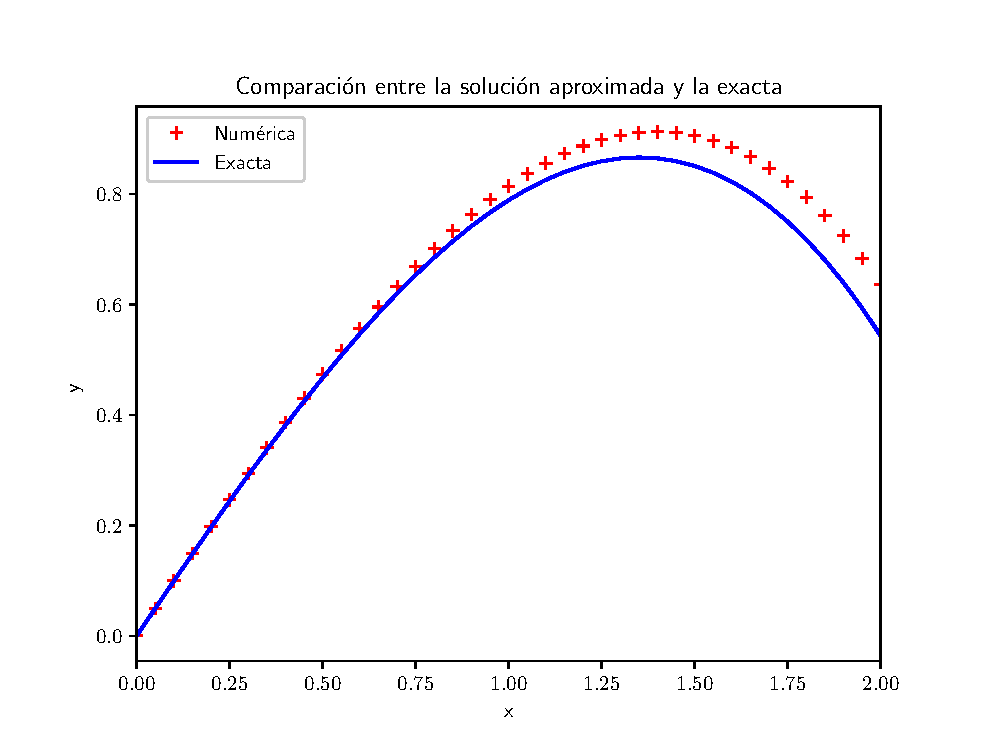
\includegraphics[scale=0.55]{Imagenes/plot_euler_ejercicio_02.eps}
\end{figure}
\end{frame}
\begin{frame}
\frametitle{Conclusión}
La porción inicial de la curva es casi una línea recta. \pause Debido a que el error de truncamiento en la solución numérica es proporcional a $\sderivada{y}$, \pause la discrepancia entre las dos soluciones es pequeña.
\\
\bigskip
\pause
A medida que aumenta la curvatura de la gráfica, también lo hace el error de truncamiento.
\end{frame}
\begin{frame}
\frametitle{Conclusión}
Es posible ver el efecto cuando cambiamos el valor de $h$, \pause ejecutando el programa con $h = 0.025$.
\\
\bigskip
\pause
Si lo hacemos, \pause \textocolor{carmine}{¿se debería reducir a la mitad el error de truncamiento?}.
\end{frame}
\begin{frame}
\frametitle{Cambiando el valor $h = 0.025$}
\begin{figure}
	\centering
	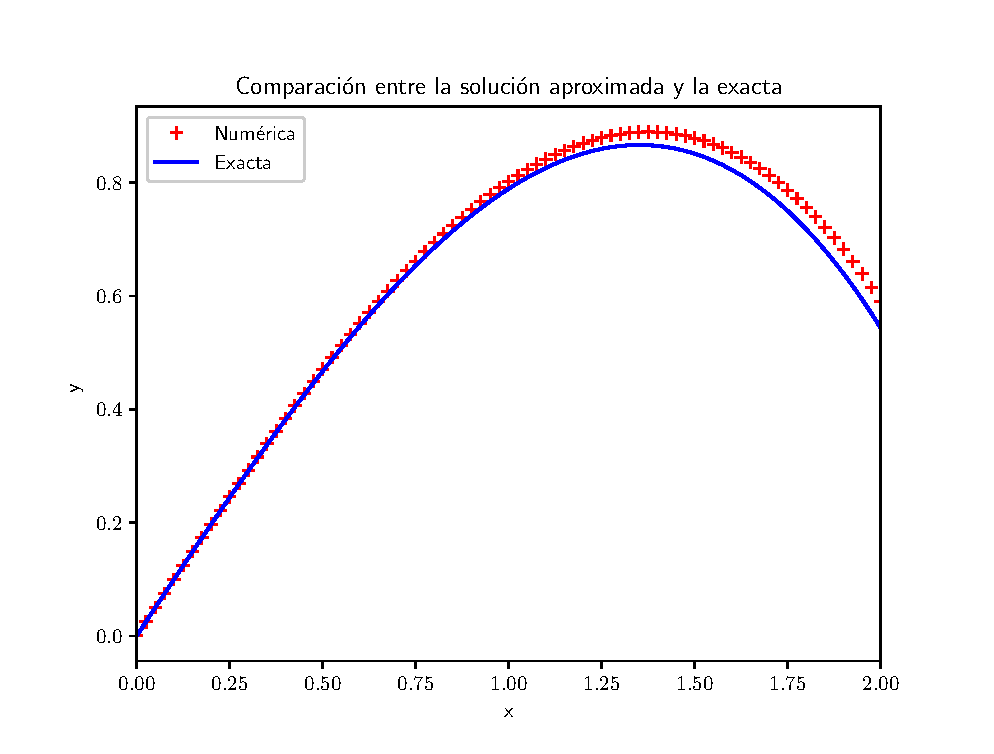
\includegraphics[scale=0.55]{Imagenes/plot_euler_ejercicio_03.eps}
\end{figure}
\end{frame}
\begin{frame}
\frametitle{Ejercicios a cuenta}
Presenta el sistema de EDO1 de la forma  de la siguientes ED:
\setbeamercolor{item projected}{bg=black,fg=white}
\setbeamertemplate{enumerate items}{%
\usebeamercolor[bg]{item projected}%
\raisebox{1.5pt}{\colorbox{bg}{\color{fg}\footnotesize\insertenumlabel}}%
}
\begin{enumerate}
\item $\ln \pderivada{y} + y = \sin x$
\item $\sderivada{y} \, y - x \, \pderivada{y} - 2 \, y^{2} = 0$
\item $\nderivada{y}{4} - 4 \, \sderivada{y} \, \sqrt{1 - y^{2}} = 0$
\item $\big( \sderivada{y} \big)^{2} = \abs{ 32 \, \pderivada{y} \, x - y^{2}}$
\seti
\end{enumerate}
\end{frame}
\begin{frame}
\frametitle{Ejercicio a cuenta}
\setbeamercolor{item projected}{bg=black,fg=white}
\setbeamertemplate{enumerate items}{%
\usebeamercolor[bg]{item projected}%
\raisebox{1.5pt}{\colorbox{bg}{\color{fg}\footnotesize\insertenumlabel}}%
}
\begin{enumerate}
\conti
\item Resuelve con el método de Euler la siguiente EDO1:
\begin{align*}
\pderivada{y} = \sin y \hspace{1cm} y (0) = 1
\end{align*}
de $x = 0$ a $0.5$, usando $h = 0.1$. Compara el resultado con lo que obtuvimos en el ejemplo dentro de esta presentación.
\end{enumerate}
\end{frame}
\subsection{Precisión y estabilidad}

\begin{frame}
\frametitle{Sobre la estabilidad del método}
Para ilustrar sobre la precisión y estabilidad del método de Euler, consideremos el siguiente problema con una EDO2:
\pause
\begin{align*}
\sderivada{y} + y = 0 \hspace{1.2cm} y (0) = y_{0}, \hspace{0.7cm} \pderivada{y} (0) = \pderivada{y}_{0}
\end{align*}
\end{frame}
\begin{frame}
\frametitle{Solución general}
La solución general de este problema es:
\pause
\begin{align*}
y (t) = A \, \sin t + B \, \cos t
\end{align*}
\pause
donde las constantes dependen de los valores particulares de $y_{0}$ e $\pderivada{y}_{0}$
\end{frame}
\begin{frame}
\frametitle{Usando la notación}
En concondarcia con la notación que hemos definido, se tiene que:
\pause
\begin{align*}
\mathbf{F} (x, \mathbf{y}) = 
\begin{bmatrix}
\pderivada{y}_{0} \\
\pderivada{y}_{1}
\end{bmatrix} =
\begin{bmatrix}
y_{1} \\
- y_{0}
\end{bmatrix}
\hspace{1.5cm}
\mathbf{y} (0) = 
\begin{bmatrix}
y_{0} \\
\pderivada{y}_{0}
\end{bmatrix}
\end{align*}
\end{frame}
\begin{frame}
\frametitle{Solución exacta}
En el caso particular de los valores iniciales:
\pause
\begin{align*}
y_{1} (0) = 0 \hspace{1cm} y_{2} (0) = 1
\end{align*}
\pause
La solución exacta a este problema, es:
\pause
\begin{align*}
y_{1} (t) = \sin t \hspace{1cm} y_{2} (t) = \cos t
\end{align*}
\end{frame}
\begin{frame}
\frametitle{Gráfica del Ejercicio 3}
\begin{figure}
	\centering
	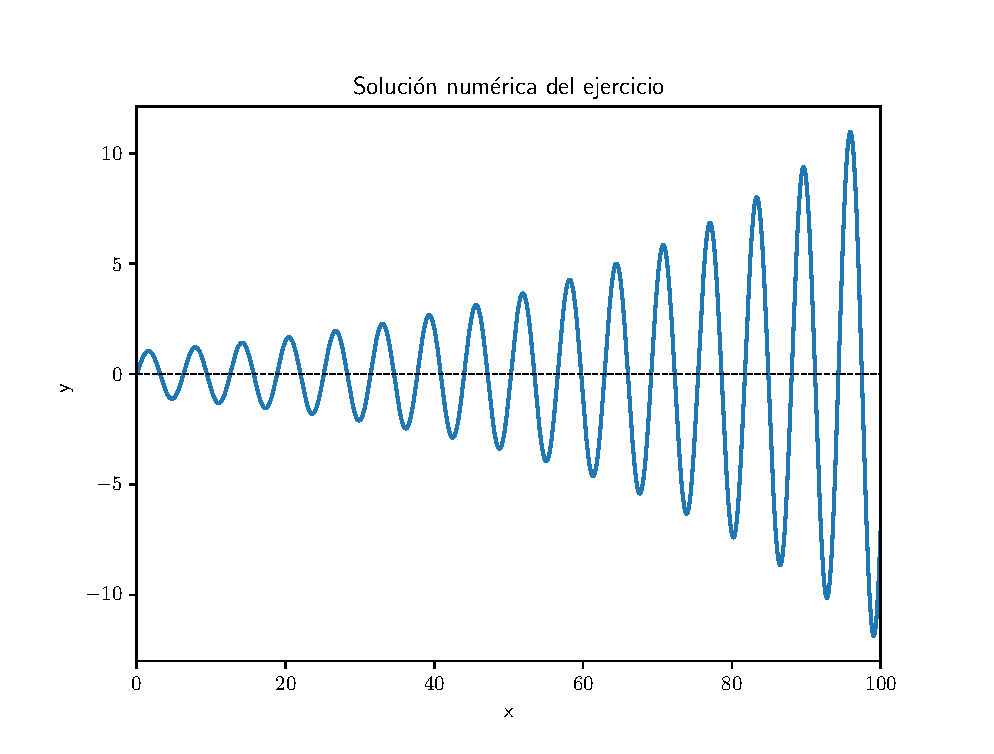
\includegraphics[scale=0.55]{Imagenes/plot_euler_ejercicio_04.eps}
\end{figure}
\end{frame}
\begin{frame}
\frametitle{La estabilidad el método de Euler}
Una indicación sobre la estabilidad numérica de la solución la proporciona la dependencia de un componente de la solución con respecto al otro, \pause concretamente, la gráfica de $y_{1}$ contra $y_{2}$. 
\\
\bigskip
\pause
Es decir, una gráfica del espacio fase.
\end{frame}
\begin{frame}
\frametitle{La estabilidad el método de Euler}
En un caso de propagación estable, se espera que la curva $y_{1}$ = $y_{1} (y_{2})$ sea un círculo cerrado de radio la unidad.
\end{frame}
\begin{frame}
\frametitle{Gráfica del Ejercicio 3}
\begin{figure}
	\centering
	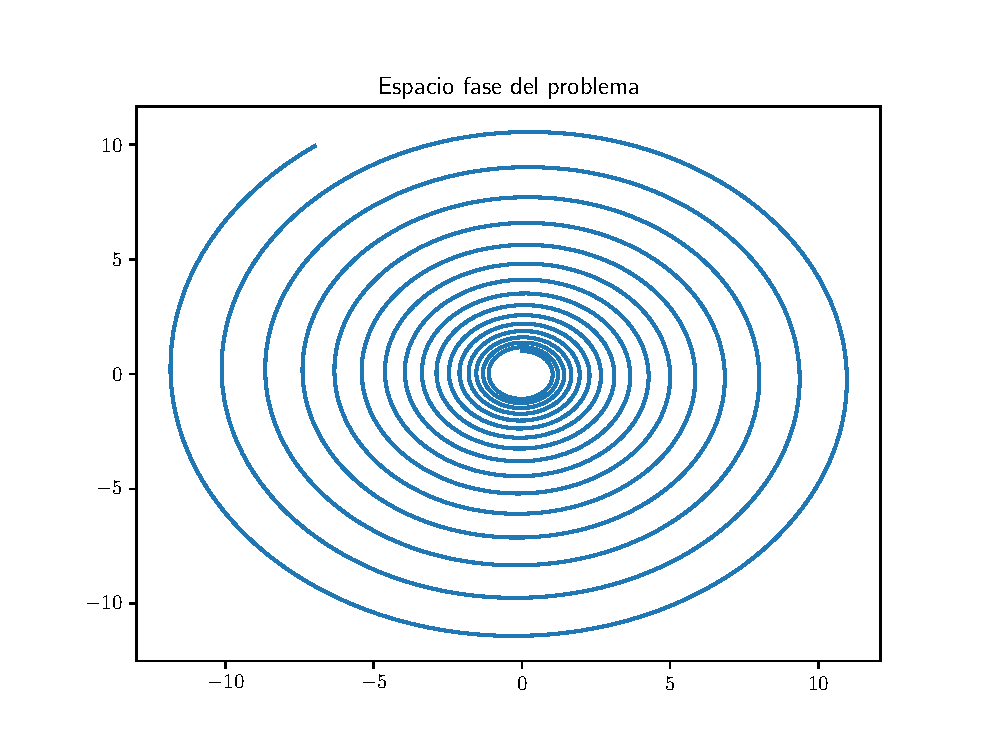
\includegraphics[scale=0.55]{Imagenes/plot_euler_ejercicio_05.eps}
\end{figure}
\end{frame}
\begin{frame}
\frametitle{Sobre el espacio fase}
Como se puede observar en la figura anterior, que representa la evolución de los perfiles en un lapso de tiempo $tmax = 100$, obtenido con un tamaño de paso de propagación $h = 0.05$, la solución obtenida por el método de Euler se aparta progresivamente del esperado comportamiento circular.
\end{frame}
\begin{frame}
\frametitle{¿Qué hacemos para mejorar?}
La respuesta a esta pregunta se tendrá cuando vemos el subtema: \pause \textocolor{ao}{métodos corrector-predictor}.
\end{frame}

\section{Métodos de Runge-Kutta}
\frame{\tableofcontents[currentsection, hideothersubsections]}
\subsection{Definición}

\begin{frame}
\frametitle{Métodos de Runge-Kutta}
La principal desventaja de los métodos de Euler es que su precisión es baja.
\\
\bigskip
\pause
Para hacer que el nivel de precisión aumente, hay que reducir $h$, pero esto genera que se lleve más tiempo en el cálculo y se propague el error por redondeo.
\end{frame}
\begin{frame}
\frametitle{Método de primer orden}
El método de Euler se clasifica como un \textocolor{red}{método de primer orden} porque su error de truncamiento acumulativo se comporta como $\order{h}$, \pause su base fue la serie truncada de Taylor:
\begin{align*}
\mathbf{y} (x + h) = \mathbf{y} (x) + \pderivada{\mathbf{y}} (x) \, h
\end{align*}
\end{frame}
\begin{frame}
\frametitle{Mejorando la precisión}
La precisión de la integración numérica se puede mejorar mucho manteniendo más términos de la serie.
\\
\bigskip
\pause
Por lo tanto, un método de n-ésimo orden usaría la serie de Taylor truncada:
\begin{align*}
\mathbf{y} (x + h) = \mathbf{y} (x) + \pderivada{\mathbf{y}} (x) \, h + \dfrac{1}{2!} \sderivada{\mathbf{y}} (x) \, h^{2} + \ldots + \dfrac{1}{n!} \nderivada{\mathbf{y}}{n} (x) \, h^{n} 
\end{align*}
\end{frame}
\begin{frame}
\frametitle{Desventaja al aumentar términos}
Pero ahora debemos derivar las expresiones para $\sderivada{\mathbf{y}}$, $\tderivada{\mathbf{y}}$, $\ldots, \nderivada{\mathbf{y}}{n}$ diferenciando repetidamente $\pderivada{\mathbf{y}} = \mathbf{F} (x, \mathbf{y})$ y escribiendo subrutinas para evaluarlas.
\end{frame}
\begin{frame}
\frametitle{Procedimiento para ahorrar trabajo}
Este trabajo adicional se puede evitar utilizando los \textocolor{ao(english)}{métodos de Runge-Kutta} \pause que también se basan en series de Taylor truncadas, pero que no requieren el cálculo de derivadas superiores de $\mathbf{y} (x)$.
\end{frame}

\section{Métodos de segundo orden}
\frame{\tableofcontents[currentsection, hideothersubsections]}
\subsection{Construyendo los métodos}

\begin{frame}
\frametitle{Desarrollo general}
Para obtener el método de Runge-Kutta de segundo orden (RK2), suponemos la integración de una expresión del tipo:
\pause
\begin{align}
\begin{aligned}
\mathbf{y} (x + h) &= \mathbf{y} (x) + c_{0} \, \mathbf{F} (x, \mathbf{y}) \, h + \\
&+ c_{1} \, \mathbf{F} \big[ x + p \, h, \mathbf{y} + q \, h \, \mathbf{F} (x, \mathbf{y}) \big] \, h
\end{aligned}
\label{eq:ecuacion_7_3_a}
\end{align}
para encontrar los parámetros $c_{0}$, $c_{1}$, $p$ y $q$, haciéndolos coincidir con la serie de Taylor:
\end{frame}
\begin{frame}
\frametitle{Serie a igualar}
\begin{eqnarray}
\begin{aligned}
\mathbf{y} (x + h) &= \mathbf{y} (x) + \pderivada{\mathbf{y}} (x) \, h + \dfrac{1}{2!} \sderivada{\mathbf{y}} (x) \, h^{2} = \\ \pause
&=  \mathbf{y} (x) + \mathbf{F} (x, \mathbf{y}) \, h + \dfrac{1}{2!} \, \mathbf{\sderivada{F}} (x, \mathbf{y}) \, h^{2}
\end{aligned}
\label{eq:ecuacion_7_3_b}
\end{eqnarray}
\end{frame}
\begin{frame}
\frametitle{Desarrollo de la derivada}
Tomemos en cuenta que:
\pause
\begin{eqnarray*}
\begin{aligned}
\mathbf{\sderivada{F}} (x, \mathbf{y}) &= \pdv{\mathbf{F}}{x} + \nsum_{i=0}^{n-1} \pdv{\mathbf{F}}{y_{i}} \, \pderivada{y}_{i} = \\ \pause
&= \pdv{\mathbf{F}}{x} + \nsum_{i=0}^{n-1} \pdv{\mathbf{F}}{y_{i}} \, F_{i} (x, \mathbf{y})
\end{aligned}
\end{eqnarray*}
\pause
donde $n$ es el número de EDO1.
\end{frame}
\begin{frame}
\frametitle{Reescribiendo la ecuación}
La ecuación (\ref{eq:ecuacion_7_3_b}) se puede escribir como:
\pause
\begin{align}
\begin{aligned}
\mathbf{y} (x + h) &= \mathbf{y} (x) + c_{0} \, \mathbf{F} (x, \mathbf{y}) \, h + \\
&+ \dfrac{1}{2} \, \bigg[ \pdv{\mathbf{F}}{x} + \nsum_{i=0}^{n-1} \pdv{\mathbf{F}}{y_{i}} \, F_{i} (x, \mathbf{y}) \bigg] \, h^{2}	
\end{aligned}
\label{eq:ecuacion_7_3_c}
\end{align}
\end{frame}
\begin{frame}
\frametitle{Revisando los términos}
Regresando a la ec. (\ref{eq:ecuacion_7_3_a}), podemos reescribir el último término usando la serie de Taylor en varias variables:
\pause
\begin{align*}
\mathbf{F} \big[ x + p \, h, \mathbf{y} + q \, h \, \mathbf{F} (x, \mathbf{y}) \big] &= \mathbf{F} (x, \mathbf{y}) + \pdv{\mathbf{F}}{x} \, p \, h + \\ 
&+ q \, h \, \nsum_{i=1}^{n-1} \pdv{\mathbf{F}}{y_{i}} \, F_{i} (x, \mathbf{y})
\end{align*}
\end{frame}
\begin{frame}
\frametitle{Ecuación obtenida}
Por lo que la ec. (\ref{eq:ecuacion_7_3_a}) se presenta como:
\pause
\begin{align}
\begin{aligned}
\mathbf{y} (x + h) &= \mathbf{y} (x) + \big[ c_{0} + c_{1} \big] \, \mathbf{F} (x, \mathbf{y}) \, h + \\
&+ c_{1} \bigg[ \pdv{\mathbf{F}}{x} \, p \, h + q \, h \, \nsum_{i=1}^{n-1} \pdv{\mathbf{F}}{y_{i}} \, F_{i} (x, \mathbf{y}) \bigg] \, h
\end{aligned}
\label{eq:ecuacion_7_3_d}
\end{align}
\end{frame}
\begin{frame}
\frametitle{Comparando las ecuaciones}
Comparando las ecs. (\ref{eq:ecuacion_7_3_c}) y (\ref{eq:ecuacion_7_3_d}), se tiene que las expresiones son idénticas si:
\pause
\begin{align}
c_{0} + c_{1} = 1 \hspace{1cm} c_{1} \, p = \dfrac{1}{2} \hspace{1cm} c_{1} \, q = \dfrac{1}{2}
\label{eq:ecuacion_7_3_e}
\end{align}
\pause
Este sistema tiene tres ecuaciones y cuatro parámetros incógnitos, \pause por lo que podemos darle cualquier valor a uno de esos parámetros.
\end{frame}
\begin{frame}
\frametitle{Métodos de solución}
Los siguientes métodos indican los valores y el nombre:
\pause
\begin{table}
\centering
\begin{tabular}{l l l l l}
$c_{0} = 0$ & $c_{1} =  1$ & $p = \dfrac{1}{2}$ & $q = \dfrac{1}{2}$ & Euler modificado \\ \hline
$c_{0} = \dfrac{1}{2}$ & $c_{1} = \dfrac{1}{2}$ & $p = \dfrac{1}{2}$ & $q = 1$ & Heun \\ \hline
$c_{0} = \dfrac{1}{3}$ & $c_{1} = \dfrac{2}{3}$ & $p = \dfrac{3}{4}$ & $q = \dfrac{3}{4}$ & Ralston \\ \hline
\end{tabular}
\end{table}
\end{frame}
\begin{frame}
\frametitle{Métodos de segundo orden}
Todas estas fórmulas se clasifican como \textocolor{blue(pigment)}{métodos de Runge-Kutta de segundo orden}, sin que ninguna fórmula tenga superioridad numérica sobre las demás.
\end{frame}

\section{Runge-Kutta de segundo orden}
\frame{\tableofcontents[currentsection, hideothersubsections]}
\subsection{El método RK2}

\begin{frame}
\frametitle{Métodos RK2}
Eligiendo el método de Euler modificado, sustityendo los parámetros correspondientes en la ec. (\ref{eq:ecuacion_7_3_a}), nos lleva a:
\pause
\begin{align}
\mathbf{y} (x + h) &= \mathbf{y} (x) + \mathbf{F} \bigg[ x + \dfrac{h}{2}, \mathbf{y} + \dfrac{h}{2} \, \mathbf{F} (x , \mathbf{y}) \bigg] \, h
\label{eq:ecuacion_7_3_f}
\end{align}
\end{frame}
\begin{frame}
\frametitle{Operaciones a realizar}
La fórmula de integración se puede evaluar convenientemente con las siguientes operaciones:
\pause
\begin{align}
\begin{aligned}
\mathbf{K}_{0} &= h \, \mathbf{F} (x, \mathbf{y}) \\
\mathbf{K}_{1} &= h \, \mathbf{F} \bigg[ x + \dfrac{h}{2}, \mathbf{y} + \dfrac{1}{2} \, \mathbf{K}_{0} \bigg] \\
\mathbf{y} (x + h) &= \mathbf{y} (x) + \mathbf{K}_{1}
\end{aligned}
\label{eq:ecuacion_07_09}
\end{align}
\end{frame}
\begin{frame}
\frametitle{Representación gráfica RK2}
\begin{figure}
    \centering
\begin{tikzpicture}[font=\small]
	\draw [->] (-0.5, 0) -- (7, 0);
	\draw [->] (-0.5, 0) -- node [pos=1, left] {$\pderivada{y} (x)$} (-0.5, 5);
	\draw [thick] (1, 2) .. controls (2.5, 3.5) and (4,4) .. (6, 4);
	\draw (7.3, -0.1) node {$x$};
	% \draw (7.2, 4.2) node {$f (x, y)$};
	\draw [dashed] (1.5, 0) -- (1.5, 2.4);
	\draw (1.3, -0.2) node {$x$};
	\draw [dashed] (5, 0) -- (5, 4);
	\draw (5, -0.2) node {$x + h$};
	\draw [pattern=north west lines, pattern color=blue] (1.5, 0) rectangle (3.3, 3.55);
	\draw [pattern=north west lines, pattern color=blue] (3.3, 0) rectangle (5, 3.55);
	\draw [fill=white] (2.2, 1.5) rectangle (2.7, 2.5) node [pos=0.5] {$\dfrac{h}{2}$};
	\draw [fill=white] (4, 1.5) rectangle (4.5, 2.5) node [pos=0.5] {$\dfrac{h}{2}$};
	\draw [<->, thick] (1.5, 1) -- (3.3, 1);
	\draw [<->, thick] (3.3, 1) -- (5, 1);
	\draw (0.5, 2.5) -- (1.5, 2.5);
	\node at (0.5, 1.3) {$f (x, y)$};
	\draw[<-] (0.7, 0) -- (0.7, 1);
	\draw[->] (0.7, 1.5) -- (0.7, 2.5);
	\draw (5, 3.55) -- (6, 3.55);
	\draw [<->] (5.6, 0) -- (5.6, 3.55);
	\node at (7.4, 2) {$f \bigg( x + \dfrac{h}{2}, y + \dfrac{\mathbf{K}_{0}}{2} \bigg)$};
	% \draw [->, thick] (5.5, 3) -- (3.5, 3);
	% \node at (7.2, 1) {Fórmula de Euler};
	% \draw [->, thick] (5.6, 1) -- (3, 1);
\end{tikzpicture}
\end{figure}
\end{frame}
\begin{frame}
\frametitle{De la gráfica anterior}
La figura anterior muestra la interpretación gráfica de la fórmula de Euler modificada para una sola ecuación diferencial $\pderivada{y} = f (x, y)$.
\\
\bigskip
La primera de las ecs. (\ref{eq:ecuacion_07_09}) produce una estimación de $y$ en el punto medio del panel mediante la fórmula de Euler:
\begin{align*}
y \bigg( x + \dfrac{h}{2} \bigg) = y (x) + f (x, y) \, \dfrac{h}{2} = y (x) + \dfrac{K_{0}}{2}
\end{align*}
\end{frame}
\begin{frame}
\frametitle{De la gráfica anterior}
La segunda ecuación luego aproxima el área del panel por el área $K_{1}$ del rectángulo rayado.
\\
\bigskip
\pause
El error aquí es proporcional a la curvatura $ (\pderivada{y})^{\prime \prime} = \tderivada{y}$ de la gráfica.
\end{frame}
\begin{frame}[allowframebreaks, fragile]
\frametitle{Código para el RK2}
\begin{lstlisting}[caption=Código que utiliza el método de RK2]
def integraorden2(F, x, y, xAlto, h):

    def run_kut2(F, x, y, h):
        K0 = h * F(x, y)
        K1 = h * F(x + h/2., y + K0/2.)
        return  y + K1
    
    X = []
    Y = []
    X.append(x)
    Y.append(y)
    
    while x < xAlto:
        h = min(h, xAlto - x)
        y = run_kut2(F, x, y, h)
        x = x + h
        X.append(x)
        Y.append(y)
    
    return np.array(X), np.array(Y)
\end{lstlisting}
\end{frame}
\begin{frame}
\frametitle{Detalle del RK2}
Los métodos de segundo orden no son populares en las aplicaciones computacionales.
\\
\bigskip
\pause
La mayoría de los programadores prefieren \textocolor{brown(web)}{fórmulas de integración de cuarto orden}, que logran una precisión dada con menos esfuerzo computacional.
\end{frame}

\subsection{Ejercicio RK2}

\begin{frame}
\frametitle{Planteamiento del ejercicio}
Con el método RK2 resuelve el siguiente problema:
\pause
\begin{align*}
\pderivada{y} = \sin y \hspace{2cm} y(0) = 1
\end{align*}
de $x = 0$ a $x = 0.5$ en pasos de $h = 0.1$.
\end{frame}
\begin{frame}
\frametitle{Notación para el ejercicio}
Ocupamos nuevamente la notación que hemos ocupado:
\begin{align*}
\mathbf{F} (x, \mathbf{y}) = 
\begin{bmatrix}
\pderivada{y}_{1}
\end{bmatrix} =
\begin{bmatrix}
\sin \, y[0]
\end{bmatrix}
\hspace{1.5cm}
\mathbf{y} (0) = 
\begin{bmatrix}
1
\end{bmatrix}
\end{align*}
\end{frame}
\begin{frame}
\frametitle{Función para estimar el error}
Considera la solución exacta de la EDO para estimar el error:
\pause
\begin{align*}
y (x) = 2 \, \cot^{-1} \left( e^{-x} \, \cot \left(\dfrac{1}{2} \right) \right)
\end{align*}
que hay que evaluar en los $x_{i}$ para obtener el valor exacto y entonces estimar el error.
\end{frame}
\begin{frame}[allowframebreaks, fragile]
\frametitle{Solución con RK2}
\begin{lstlisting}[caption=Código para resolver con RK2 el ejercicio]
from metodosDirectos import integraorden2
from prettytable import PrettyTable
import numpy as np

def f(x, y):
	f = np.zeros(1)
	f[0] = np.sin(y)
	return f

x = 0.0
xAlto = 0.5
y = np.array([1.])
h = 0.1

tabla = PrettyTable()
tabla.field_names = ['x', 'Aproximación']

X, Y = integraorden2(f, x, y, xAlto, h)

for i in range(len(X)):
	tabla.add_row(['%1.1f' % X[i],'%1.8f' % Y[i]])

print(tabla)
\end{lstlisting}
\end{frame}
\begin{frame}
\frametitle{Tabla con los valores}
En la siguiente tabla se presentan los resultados obtenidos y se estima el error relativo con respecto al valor exacto de la solución.
\\
\bigskip
\pause
Esos valores los obtenemos al evaluar los $x_{i}$ en la solución exacta.
\end{frame}
\begin{frame}
\frametitle{Tabla con los valores}
\begin{table}
\centering
\renewcommand*{\arraystretch}{0.9}
\begin{tabular}{ c c c}
$x$ & Aproximación & Error relativo \\ \hline
$0.0$ & $1.00000000$ & $0.000000e+00$ \\ \hline
$0.1$ & $1.08634520$ & $1.054549e-05$ \\ \hline
$0.2$ & $1.17681165$ & $8.455224e-06$ \\ \hline
$0.3$ & $1.27082361$ & $6.723609e-06$ \\ \hline
$0.4$ & $1.36766006$ & $3.383559e-05$ \\ \hline
$0.5$ & $1.46647408$ & $7.007514e-05$ \\ \hline
\end{tabular}
\end{table}
\end{frame}

\end{document}